\documentclass[twoside]{article}
\usepackage[a4paper]{geometry}
\geometry{verbose,tmargin=2.5cm,bmargin=2cm,lmargin=2cm,rmargin=2cm}
\usepackage{fancyhdr}
\pagestyle{fancy}

% nastavení pisma a~češtiny
\usepackage{lmodern}
\usepackage[T1]{fontenc}
\usepackage[utf8]{inputenc}
\usepackage[czech]{babel}

% odkazy
\usepackage{url}

\usepackage{float}
% vícesloupcové tabulky
\usepackage{multirow}
\usepackage{listings}
\usepackage{xcolor}
\usepackage{amssymb}
\usepackage{gensymb}
\usepackage{bbold}
\usepackage{amsmath}
\usepackage{siunitx}
\usepackage{mathtools}
\usepackage{commath}

% vnořené popisky obrázků
\usepackage{subcaption}

% automatická konverze EPS 
\usepackage{graphicx} 
\usepackage{epstopdf}
\epstopdfsetup{update}

\graphicspath{{./images}}

% odkazy a~záložky
\usepackage[unicode=true, bookmarks=true,bookmarksnumbered=true,
bookmarksopen=false, breaklinks=false,pdfborder={0 0 0},
pdfpagemode=UseNone,backref=false,colorlinks=true] {hyperref}


% Poznámky při překladu
\usepackage{xkeyval}	% Inline todonotes
\usepackage[textsize = footnotesize]{todonotes}
\presetkeys{todonotes}{inline}{}

%https://tex.stackexchange.com/questions/2783/bold-calligraphic-typeface
\DeclareMathAlphabet\mathbfcal{OMS}{cmsy}{b}{n}

% enumerate zacina s pismenem
\renewcommand{\theenumi}{\alph{enumi}}

% smaz aktualni page layout
\fancyhf{}
% zahlavi
\usepackage{titling}
\fancyhf[HC]{\thetitle}
\fancyhf[HLE,HRO]{\theauthor}
\fancyhf[HRE,HLO]{\today}
 %zapati
\fancyhf[FLE,FRO]{\thepage}

% údaje o autorovi
\title{VSY - Tester reakce A - dokumentace}
\author{Vojtěch Michal}
\date{\today}

%customize code listing
\definecolor{codegreen}{rgb}{0,0.6,0}
\definecolor{codegray}{rgb}{0.5,0.5,0.5}
\definecolor{codepurple}{rgb}{0.58,0,0.82}
\definecolor{backcolour}{rgb}{0.95,0.95,0.92}

\lstdefinestyle{mystyle}{
    backgroundcolor=\color{backcolour},   
    commentstyle=\color{codegreen},
    keywordstyle=\color{magenta},
    numberstyle=\tiny\color{codegray},
    stringstyle=\color{codepurple},
    basicstyle=\ttfamily\footnotesize,
    breakatwhitespace=false,         
    breaklines=true,                 
    captionpos=b,                    
    keepspaces=true,                 
    numbers=left,                    
    numbersep=5pt,                  
    showspaces=false,                
    showstringspaces=false,
    showtabs=false,                  
    tabsize=2
}

\lstset{style=mystyle}

\begin{document}

\maketitle

Cílem úlohy je realizovat tester rychlosti reakce uživatele. Mačkáním a uvolňováním tlačítka má uživatel reagovat na změny stavu indikátorové LED.
Po testu dostane uživatel zpětnou vazbu, zda zareagoval ve správný okamžik, nebo příliš pozdě či brzy.

\section{Chování}
\label{sec:chovani}

Základem chování aplikace je jeden test. Test je zahájen buď bezprostředně po startu, nebo je možné jej zahájit po ukončení předchozího testu. Test se skládá z několika fází.
\begin{enumerate}
    \item \textit{Příprava:} Svítí žlutá LED. Uživatel je vyzván ke stisknutí tlačítka. Pokud tak neučiní do patnácti vteřin, test je ukončen se záporným výsledkem 
    (uživatel je tak unaven, že ani nebyl schopen zareagovat na přípravu). Když uživatel stiskne tlačítko, začne hlavní tělo testu.
    \item \textit{Prodleva:} Stále svítí žlutá LED, uživatel musí držet tlačítko stisknuté. Zařízení čeká náhodnou dobu mezi 400 ms a 10 s. 
    Po skončení odpočtu zhasne žlutá LED a uživatel musí co nejrychleji uvolnit stisknuté tlačítko.
    \item \textit{Vyhodnocení:} Bliká buďto zelená nebo červená LED. Zařízení tak signalizuje, že uživatel buďto test splnil, nebo se mu test nezdařil
    (uvolnil tlačítko příliš pozdě či brzy).
\end{enumerate}

Po ukončení testu (z fáze \textit{Vyhodnocení}) lze test kdykoli znovu zahájit pomocí dlouhého stisku tlačítka (alespoň po dobu jedné sekundy).



\section{Pinout}

Úloha počítá s přiřazením pinů mikrokontroleru uvedeným v tabulce \ref{table:pinout}. Tlačítko není potřeba v případě desky Nucleo připojovat,
protože je přímo vestavěno na desce (modré tlačítko s popisem \textit{USER}).
Diody je potřeba připojit externě pro získání plného zážitku z aplikace. Pakliže by nebyla možnost k desce připojit diody externí,
je možné využít fallback LED připojenou na PA5, která je umístěná přímo na Nucleu.

Fallback LED spojuje roli všech tří hlavní LED, stav průběhu testu je možné rozlišit na základě sledování periody blikání.
Rychlé blikání odpovídá špatné reakci od uživatele, pomalé blikání signalizuje, že uživatel zareagoval správně.
Konstantní svit signalizuje přípravu či probíhající test. Viz \ref{sec:chovani} pro detailní popis logiky aplikace.

\begin{table}[htbp]
    \centering
    \begin{tabular}{c|c|c}
        signál & pin MCU & pin Nuclea \\ \hline
        tlačítko & PC13 & -- \\
        červená LED & PA0 & A0 \\
        žlutá LED & PA1 & A1 \\
        zelená LED & PA4 & A2 \\
        fallback LED & PA5 & --
    \end{tabular}
    \caption{Piny využívané aplikací}
    \label{table:pinout}
\end{table}

\newpage
\section{Příklad signalizace}

Na obrázku \ref{fig:priprava} je rozsvícena žlutá LED -- uživatel se má připravit k testu stiskem tlačítka.\\
Na obrázku \ref{fig:bad} bliká červená LED, protože uživatel nezvládl správně zareagovat během testu.
Například pustil tlačítko příliš brzy, nebo naopak příliš pozdě.\\
Na obrázku \ref{fig:pochvala} bliká zelená LED - uživatel správně zakončil test a je oprávněn řídit auto a těžké stroje.

\begin{figure}[htbp]
    \centering
    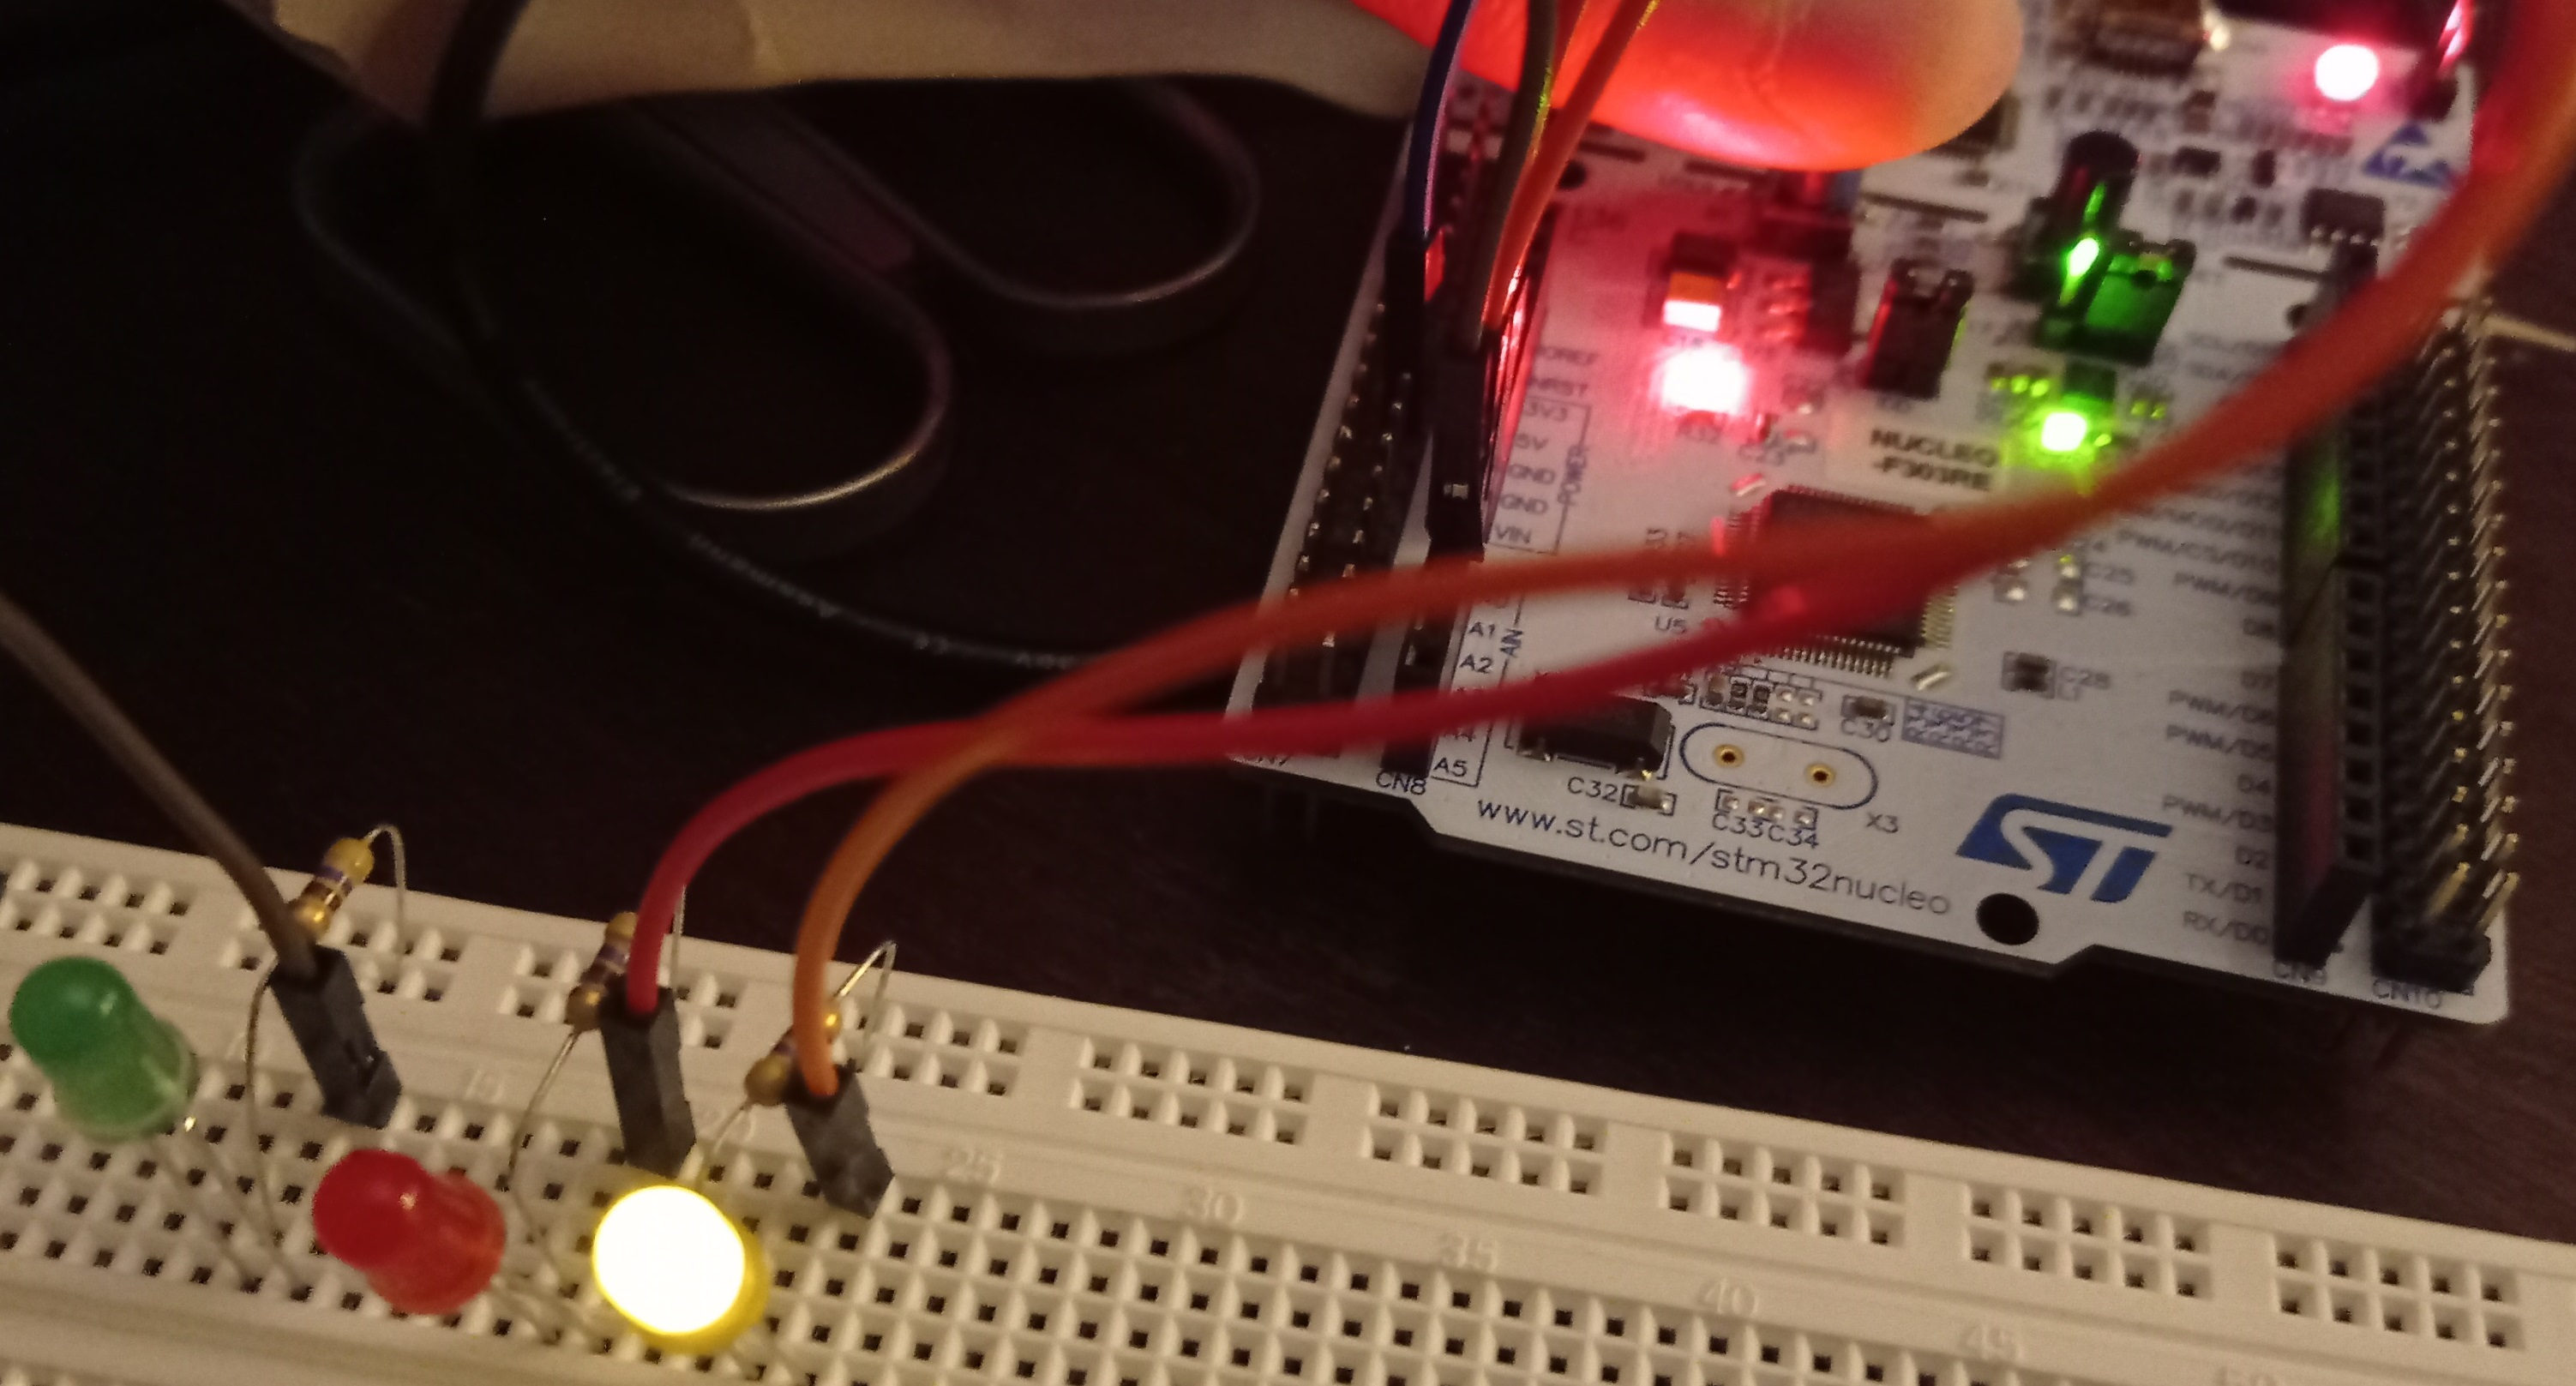
\includegraphics[height=0.2\textheight]{priprava.jpg}
    \caption{Výzva \textit{připrav se!}}
    \label{fig:priprava}
\end{figure}

\begin{figure}[htbp]
    \centering
    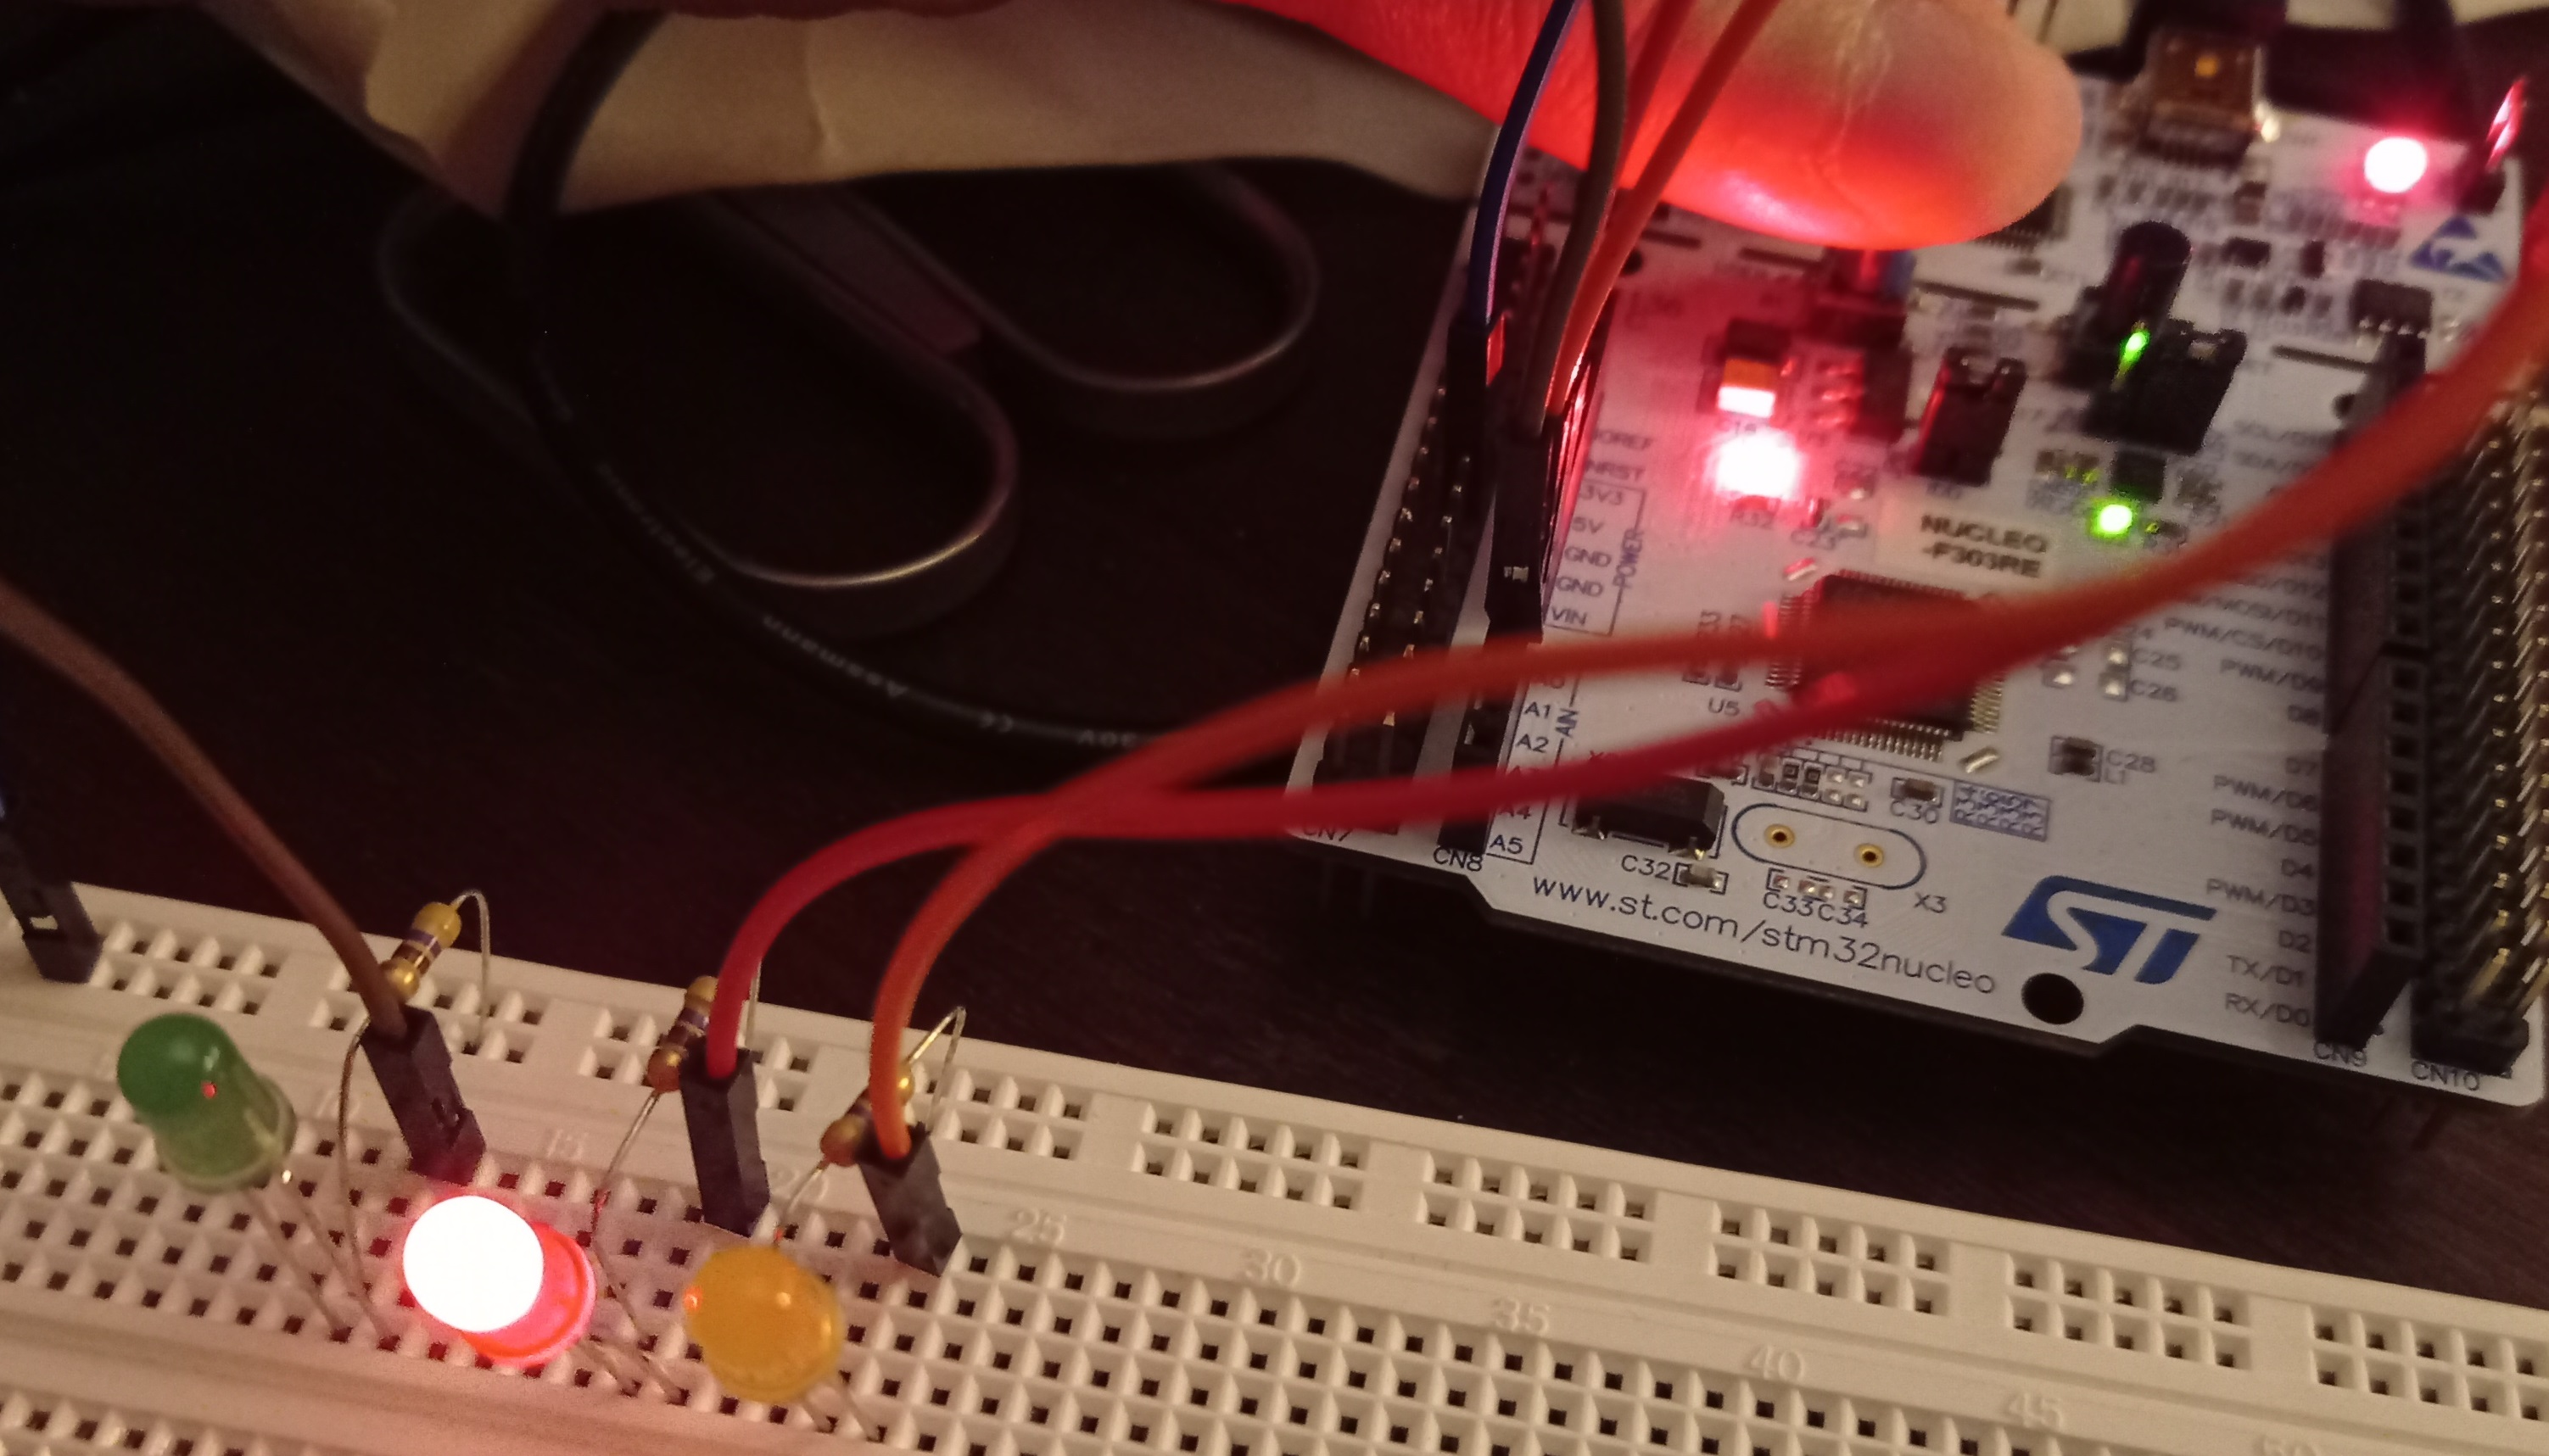
\includegraphics[height=0.2\textheight]{bad.jpg}
    \caption{Signalizace nesprávné reakce uživatele (tlačítko bylo drženo příliš dlouho)}
    \label{fig:bad}
\end{figure}

\begin{figure}[htbp]
    \centering
    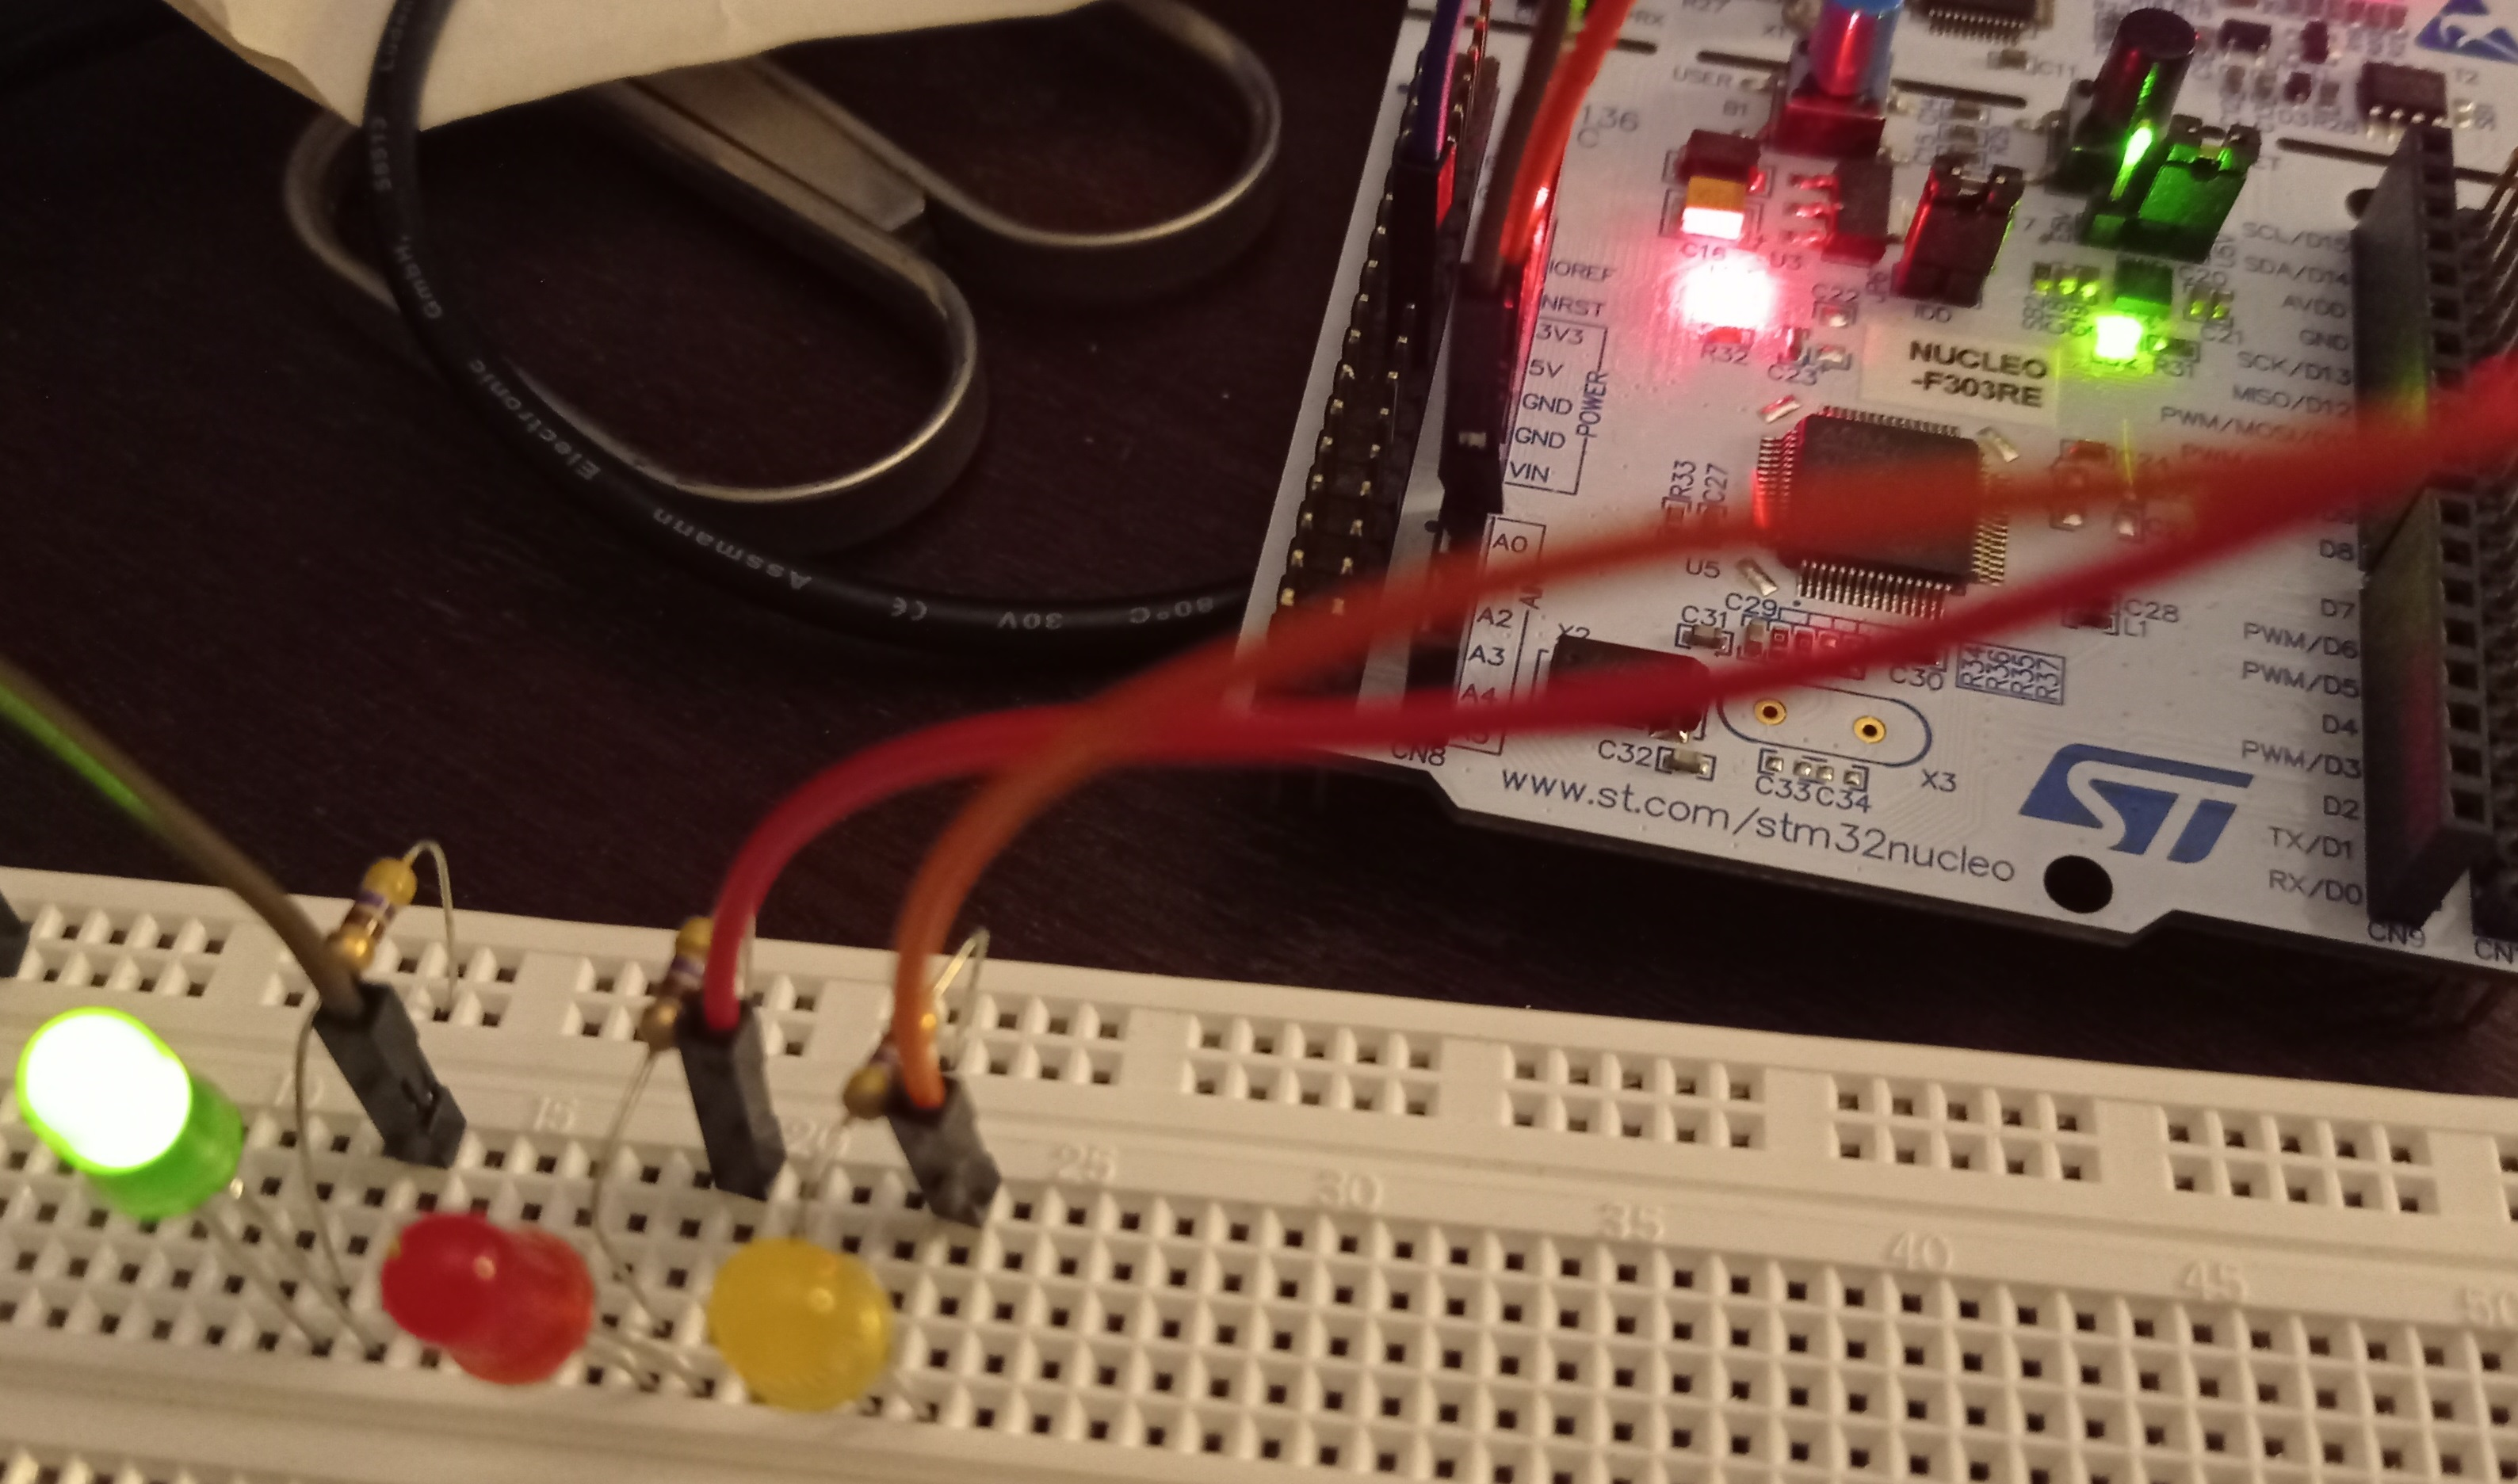
\includegraphics[height=0.2\textheight]{pochvala.jpg}
    \caption{Signalizace správné reakce uživatele}
    \label{fig:pochvala}
\end{figure}



\end{document}